Service robots are invading human lives. They are increasingly used in environments such as houses, airports, hospitals, and offices for performing navigation, transportation, and manipulation tasks. 
The World Robotic Survey~\cite{wrs:online} estimated 35 million indoor service robots to be sold by 2018, accumulating a sales value of \$12 billion since 2015. 
The global sales of household and personal robots is expected to grow by 23.5\% per year~\cite{sheng:online}. 
This increase is accompanied with huge progress in robot technology, especially in image processing, planning, control, and collaboration. Software engineering is key to sustaining this new technology.

A robot typically performs specialized tasks; however, some tasks are highly complex and require a team of robots, whose capabilities (e.g., perception, manipulation, and actuation) are coordinated and supervised. 
Such teams also need to adapt to changes, such as of the environment, of the desired tasks, or of the robot (e.g., hardware failures). 
These demands drive the complexity of robot control software relying on appropriate software architectures. 
To tackle this complexity, we need to rethink design processes~\cite{Lee2008} by properly managing system integration and raising the abstraction levels, addressing qualities like evolvability~\cite{Perez2008}, configurability~\cite{Gamez2013563}, scalability, power consumption, and dependability.

Figure~\ref{fig:overview} depicts an overview of the work being developed for this project.
There is an evident difference between two different approaches in robotic practices, that is when the robotic application puts to work an unique robot or a team of them. 
This division also splits the research schedule of this project in terms of time, as explained in the following.
The ``Single robot" subdivision of the overview represents the work already achieved and work in progress to be achieved in the near future.
This subdivision contains the block of the \emph{Software Architecture}, which is at the same time contained in the \emph{Software Platform} block.
The last mentioned block represents an additional layer for integrating the tools developed by researchers.
Our platform must also be able to be customized by means of \emph{configuration facilities}, which provide the required tools for configuring the basic platform both at design and run-time.

On the other hand, the future work that will be tackled once the single robot contents are already addresses is group in the subdivision of ``Multi robot".
The main expected outcome of this subdivision is to achieve the orchestration of a deployed team of potentially heterogeneous robots.
In order to do so, issues as \emph{Emergent properties} ~\cite{DeAngelis2015,DeAngelis2016} and selecting the most suitable \emph{Collaborative strategy} \sergio{needed citation} must be addressed.

\begin{figure}[!t]
\begin{center}
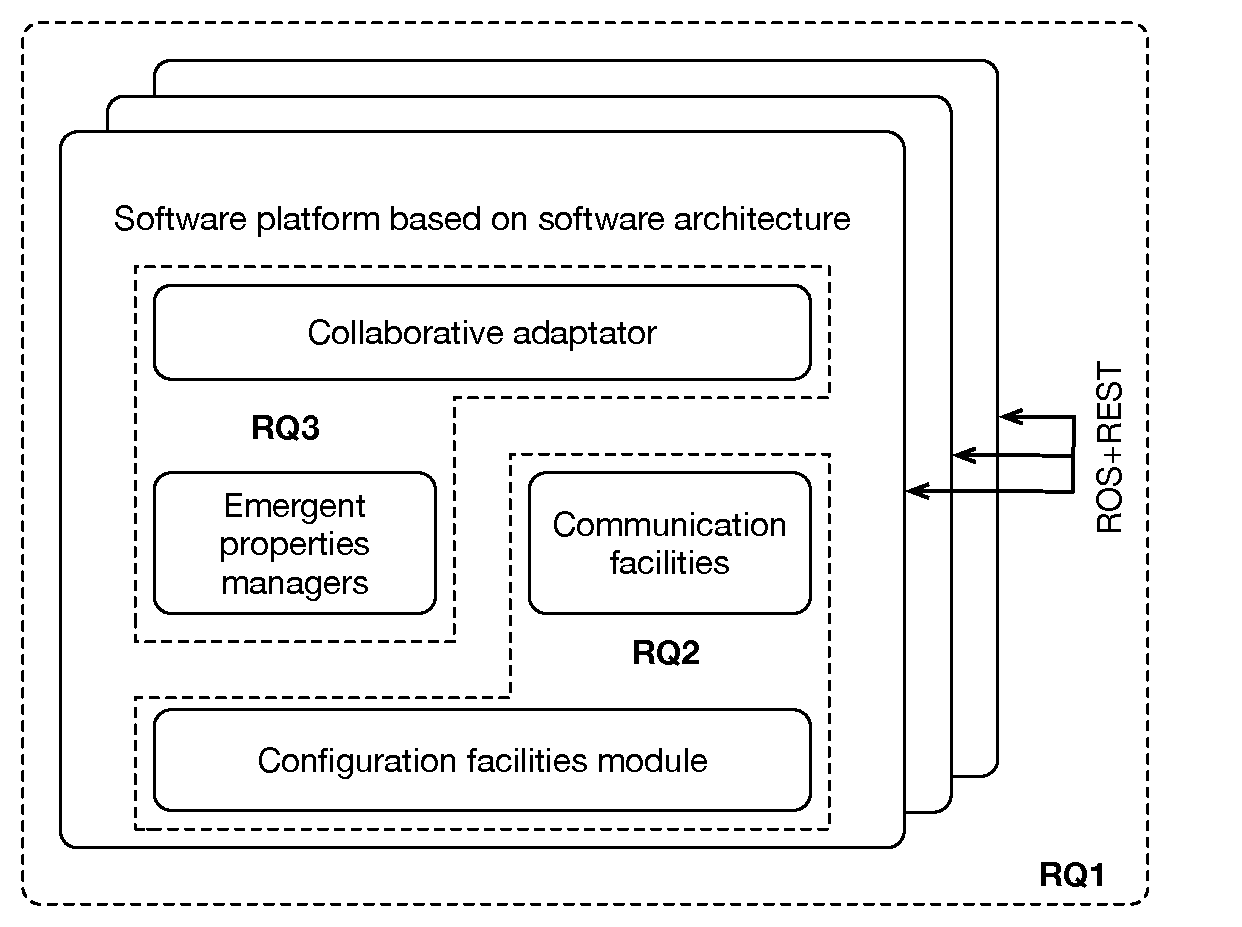
\includegraphics[width=1\linewidth]{Figures/research.pdf}
\caption{Overview of this PhD project.}
\label{fig:overview}
\end{center}
\end{figure}

\textbf{Research Questions.} 
In this project we divide robot applications between single-robot and multi-robot approaches.
For this reason, we state the following research questions:
\begin{itemize}
\item[RQ1] Which are the software engineering practices for single and multi-robotic systems? 
\item[RQ2] Which are the applicable strategies to manage an heterogeneous robotic application?
\end{itemize}

\textbf{Contributions.} 


\textbf{Organization.} 
In Section~\ref{sec:related}, we introduce different works with a similar scope and position our research.
Section~\ref{sec:approach} describes the research approach of the current work.
Then, the next sections present the current state of our work in Section~\ref{sec:current}, future work and planned directions in Section~\ref{sec:future} and it concludes with Section~\ref{sec:conclusion} with final remarks.